\documentclass{article}
\usepackage{fullpage}
\usepackage{hyperref}
\usepackage{graphicx}
\usepackage{titling}

\setlength{\droptitle}{-2cm}

\title{Will I Reply?}
\author{Anita Lacea (alacea at stanford dot edu)\\Jonathan Wheeler (jamwheel at stanford dot edu)}
\date{\today}

\begin{document}
\maketitle
\vspace{-1cm}
\begin{center}
\href{https://github.com/jondoesntgit/willireply}{https://github.com/jondoesntgit/willireply}
\end{center}

\section{Task Definition}
According to one study, business users receive about 140 emails per day, and send about 43 emails per day.\cite{emailstatistics} If we assume that half of the emails that business users send are in response to another email, then only 15\% of emails need a response and the other 85\% are either informational, or require some other action not in the form of an email reply. Work has been done in classifying emails into types calls for papers\cite{learningrulesthatclassifyemail}, spam\cite{filteringjunkemail}, and other so-called ``interesting email''\cite{emailclassification}. Various patents exist disclosing techniques to classify emails\cite{Goodman:2014ug,Bellegarda:2010wk,Romero:2005vs}, and one patent specifically discloses a means of predicting actions (such as replying, forwarding, and deleting) that a user may execute given a new email\cite{Weber:2012tv}.

We propose building an artificial intelligence that trains on your personal email history (or a combination of your email history with other users' emails it has trained on), and then predicts whether you will respond to some arbitrary future email that you receive.
\footnote{Note, that we may also consider using some much much larger datasets as well, like the Enron Corpus\cite{enroncorpus}} The input is an email (fetched via python's standard imaplib library). 
The output is a 1 if the email was or is expected to be replied to, and 0 otherwise. 
In the training set, the label is assigned by searching through a user's ``Sent Email'' folder, and searching for emails where the ``Reply-Id'' matches the ``Message-Id'' of an email in the user's ``Archive'' or ``Inbox'' folder. 
This algorithm can be integrated with another service (like push notifications on your phone) so that you only get notified when you receive an email from someone who is expecting a reply. 
You can then batch the rest of your non-time critical email together such that you process it daily. 
From the outside, users will infer from your rapid responses that you are always checking your email, when in reality, you are only responding to perhaps the 15\% of emails that require immediate responses.

\begin{center}
$\vcenter{\hbox{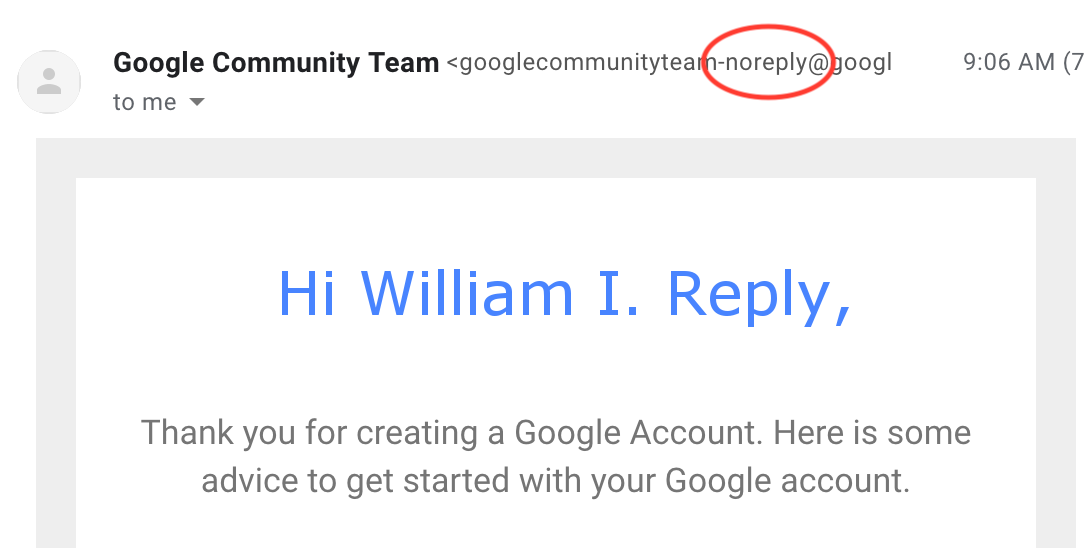
\includegraphics[height=1.5in]{no_reply.png}}} \rightarrow 0 \hspace{3em} 
\vcenter{\hbox{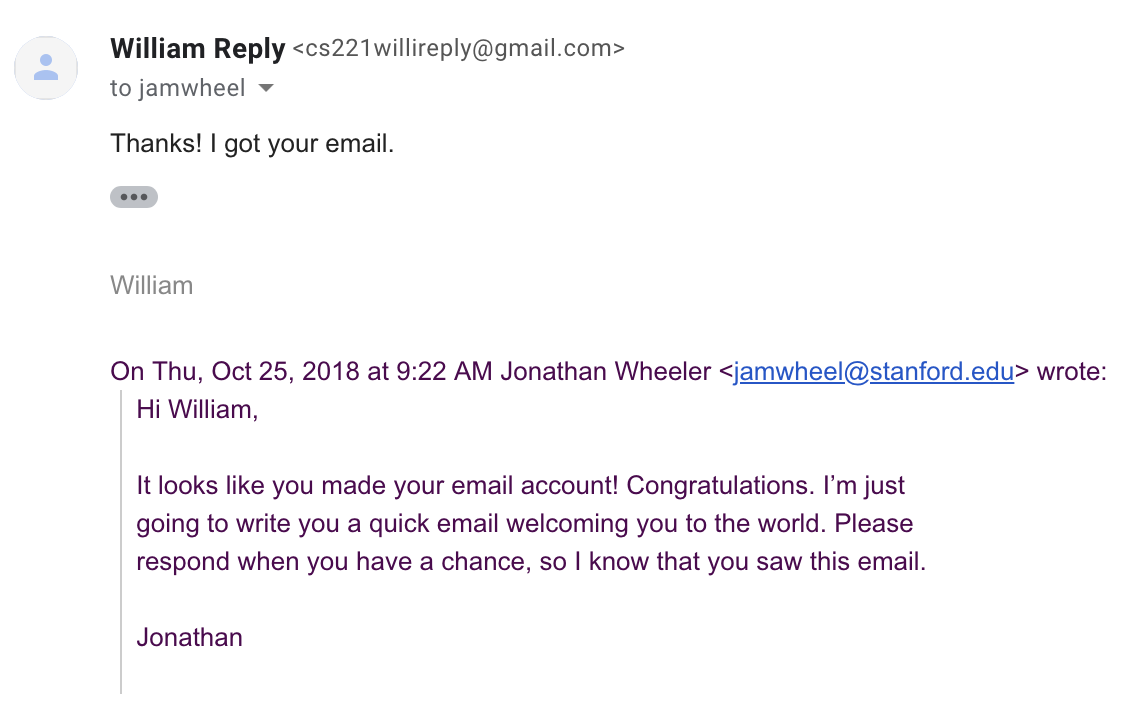
\includegraphics[height=1.5in]{reply_screenshot.png}}} \rightarrow 1 $
\end{center}

The overall approach to solving this problem will include machine learning. Various feature extractors, loss functions, and regression models will be considered over a range of experiments. Different datasets, made up of either individual users or groups of users will also be considered to see how the model needs to change when analyzing each individuals' email policies.

%\subsection{Evaluation}
Binary classifiers are often characterized by their `precision' and `recall' parameters. In our case, the precision of the `reply' label will tell us how often a prediction that we would reply to an email was correct, and the recall of the `reply' label will tell us what percentage of the emails that require a response are correctly being identified. Because we get a lot of spam (about 85\% of email is estimated not to need a reply), the precision and recall of the `no reply' label will always be quite high, and we are not interested in optimizing these parameters.

Recall and precision are both important, and so our metric will include a component of both, but the reply recall is more important for our algorithm. The penalty for failing to respond to an important email is greater than the penalty lost reading an email that does not require a response. In this case, we might use an $F_\beta$ metric\cite{fbetawikipedia}. For $\beta = 1$, precision and recall are weighted equally. For $\beta > 1$, recall is weighted more heavily. We arbitrarily set $\beta = 2$, to make recall twice as important as precision. This is the overall metric that we use to evaluate our performance. $F_2 = 0$ is the worst case scenario, $F_2 = 1$ is the best case scenario.

\section{Data and Experiments}
An initial experiment was conducted by using a sample of the 200 most-recent emails sent to jonathan.m.wheeler@gmail.com.
Out of 200 emails, 28 emails were responded to.
We used sklearn's linearregression model, and for a feature extractor, created a sparse vector of senders.
The model trained on the first 100 emails, and tested on the second 100 emails with an $F_2$ score of 42\%. 

One of Jonathan's colleagues (who has some knowledge out his personal life), read each of the 200 emails, and labeled 17 emails she believed he would respond to. Her F2 score was 15.5\%.

\section{Analysis}
The fact that a human oracle who is familiar with a user's personality cannot predict as accurately as our simple baseline test is somewhat surprising. Upon closer inspection, it was found that Jonathan frequently responded to a GitHub listserv that his colleague did not expect him to reply to. As a result, she did not mark label these as `reply', and her recall performance was impacted. The baseline test was able to see this pattern in the training set, and adapted accordingly.

\section{Challenges}
Every user has different email habits. Some users sign up to more marketing, and others keep their inboxes sparse. Some users are more likely to respond with short phrases like ``thanks'' or ``sounds good,'' whereas other users may choose not to. Some users prefer to use email for all communication, while other users may only use it for certain applications like business with external colleagues. Because each user's style is different, it is difficult to use a fit from user A's history to predict how user B will behave.

A stretch goal might include adding additional features to the algorithm that attempt to infer something about the user's habits when using emails. From that analysis, a model that is trained from user A's dataset could be adjusted by a second algorithm that knows something about user B's personality and preferences. Possible areas to explore solutions include:

\begin{itemize}
\item Determining features that are common from user-to-user, and which ones are unique, and finding ways to adapt models for each user.
\item Determining whether the user frequently responds using short phrases like ``thanks!'', ``sounds good''. This can be used to infer the user's email-use style, and adjusting models trained on other users' styles accordingly.
\end{itemize}

There are other things we may explore. A user's preferences may change over time. Reinforcement learning, or some method of discounting email habits from several years ago, could help the data to be more accurate for how a user is about to respond to new emails. Also, the model could be fine-tuned to predict whether the user will respond immediately, or will respond in a few days

\bibliography{../bibliography} 
\bibliographystyle{ieeetr}

\end{document}
